\begin{frame}{Paper Review - CBBA Guarantees}
    \begin{theorem}[Convergence of CBBA]
        Provided DMG scoring functions and synchronized consensus over a static communication network
        \begin{enumerate}
            \item CBBA produces the same solution as the sequential greedy algorithm (SGA)
            \item Convergence time is bounded above by $N_{\text{min}} \cdot D = \min \{N_t, N_u\cdot L_t\} \cdot D$ with network diameter $D$
        \end{enumerate}
    \end{theorem}
    \begin{columns}
    \begin{column}{0.7\textwidth}
    \pause
    \hspace*{16pt} Proof summary:
    \begin{itemize}
        % \item Bundle construction in CBBA is equivalent to the task selection in SGA (greedy approach)
        \item Bundle construction in CBBA $\equiv$ task selection in SGA (greedy approach)
        \item From DMG, no robot can place a higher bid in later iterations of CBBA. \pause
        \begin{itemize}
            \item $k$ iterations (where $k\le D$) of CBBA consensus lead to $k$-hop neighbors of robot $i^*$ to agree that robot $i^*$ is assigned to task $j^*$
        \end{itemize}
        \pause
        % \item Convergence time follows since the total number of assignments needed for convergence is $N_{\text{min}}$
        \item Convergence time follows since the total number of tasks needed for assignment is $N_{\text{min}}$
    \end{itemize}
    \end{column}
     % the CBBA bundle construction phase and task selection in SGA are equivalent procedures. By DMG, no robot can place a higher bid in later iterations. Thus, $k$ iterations (where $k\le D$) of CBBA conflict resolution procedures lead to $k$-hop neighbors of robot $i^*$ to agree that robot $i^*$ is the winning robot for task $j^*$. The convergence time follows since the total number of assignments needed for convergence is $N_{\text{min}}$.

    \begin{column}{0.4\textwidth}
        \begin{figure}
        \onslide<2->
        \centering
    
        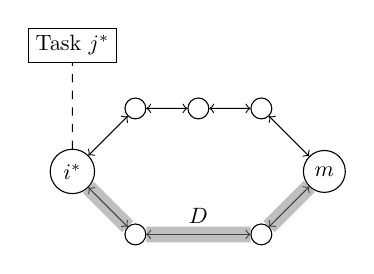
\begin{tikzpicture}[scale=0.8, transform shape]
        % Define the nodes
        \node[draw, circle] (i) at (1,0) {$i^*$};
        \node[draw, circle] (a) at (2,1) {};
        \node[draw, circle] (b) at (2,-1) {};
        \node[draw, circle] (c) at (4,1) {};
        \node[draw, circle] (d) at (4,-1) {};
        \node[draw, circle] (e) at (3,1) {}; % New node
        \node[draw, circle] (j) at (5,0) {$m$};
        \node[draw, rectangle] (task) at (1,2) {Task $j^*$}; % Square node for task
    
        % Draw the edges
        \draw[<->] (i) -- (a);
        \draw[<->] (i) -- (b);
        % \draw (a) -- (c);
        \draw[<->] (b) -- (d);
        \draw[<->] (c) -- (j);
        \draw[<->] (d) -- (j);
        \draw[<->] (a) -- (e);
        \draw[<->] (c) -- (e);
        \draw[dashed] (i) -- (task); % Dashed line to task node
    
        % Highlight the diameter path
        \draw[line width=2mm, gray, opacity=0.5] (i) -- (b) -- (d) -- (j);
    
        % Add labels
        \node at (3,-0.7) {$D$};
    \end{tikzpicture}
        \caption{Network diameter $D$}
    \end{figure}
    \end{column}
    \end{columns}
    % Proof idea: Auxilary lemmas show that CBBA and SGA iterations are equivalent, i.e., they give similar bids on tasks and a similar sequence of tasks in the bundle at every iteration.  
\end{frame}


\begin{frame}{Paper Review - CBBA Guarantees}
    \begin{theorem}[Optimality of CBBA]
        Provided DMG scoring functions and accurate situational awareness, CBBA guarantees 50\% optimality for the MRTA.
    \end{theorem}
    \textbf{Scratch}: 
    \begin{itemize}
        \item CBBA $\equiv$ SGA. Consider $L_t=1$, i.e., CBAA. \pause
        \item At iteration $k\le N_{\text{min}}$, SGA chooses a (robot,task) assignment pair $\left(i^*_{k}, j^*_{k}\right)$ greedily \pause
        \item Rearrange robot/task indices appropriately s.t. $\left(i^*_{k}, j^*_{k}\right) = (k,k)$. E.g., for 2 robot 2 task case ($N_{\text{min}} = 2$),
        \visible<3>{
        \begin{figure}
            \centering
            {
            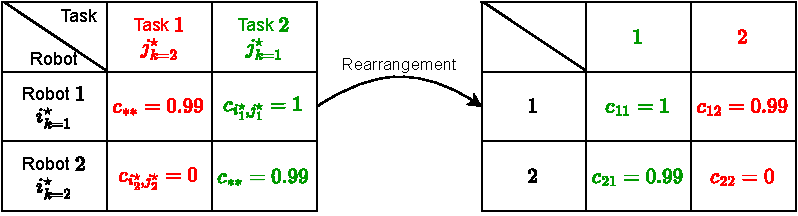
\includegraphics[width=0.85\linewidth]{Figures/2_robot_2_task.pdf}}
        \end{figure} }
        \item The SGA solution is $SGA =\sum_{i=1}^{N_{\text{min}}} c_{ii}$ (in this example $SGA=1$)
        
    \end{itemize}
\end{frame}

\begin{frame}{Paper Review - CBBA Guarantees}
     \begin{figure}
        \centering
        {
        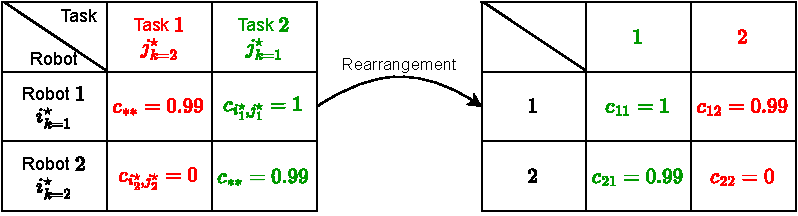
\includegraphics[width=0.8\linewidth]{Figures/2_robot_2_task.pdf}}
    \end{figure}
    \begin{itemize} 
    \item The SGA solution is $SGA =\sum_{i=1}^{N_{\text{min}}} c_{ii}$ (in this example $SGA=1$) \pause
    \item Since tasks are chosen greedily, we have,
    \begin{subequations}
        \begin{align}
        & c_{ii}\ge c_{jj}, \quad \text{if } i< j \\
        & c_{ii}\ge c_{ij}, \quad \forall i \quad \forall j > i \quad \text{``row-wise"} \\ 
        & c_{ii}\ge c_{ji}, \quad \forall i \quad \forall j > i \quad \text{``column-wise"}
        \end{align}
    \end{subequations}
    \pause
    \item The idea of the proof is to look at the worst case, i.e., variations in the assignments cause the largest improvement in objective value by swapping assignments, i.e., Eq. (2b),(2c) are equalities.
    \pause
    \begin{itemize}
        \item Notice the optimal solution for this example (which is almost worst case) is by swapping tasks between robots, which gives $OPT=0.99+0.99=1.98$ 
    \end{itemize}
    \end{itemize}
\end{frame}

\begin{frame}{Paper Review - CBBA Guarantees}
    \begin{itemize} 
        \item This worst case analysis can be extended to more robots/tasks, where again equality holds for  Eq. (2b),(2c), i.e., 
        \begin{subequations}
            \begin{align}
            & c_{ii} = c_{ij}, \quad \forall i \quad \forall j > i \quad \text{``row-wise"} \\ 
            & c_{ii} = c_{ji}, \quad \forall i \quad \forall j > i \quad \text{``column-wise"}
            \end{align}
        \end{subequations}
        \item Moreover, a swapping assignment policy where the first $\text{ceil}(N_{\text{min}}/2)$ robots and the next $\text{floor}(N_{\text{min}}/2)$ robots swap assignments, resulting in the largest gain for the latter robots, which gives the optimal solution, i.e., 
        \begin{equation}
            OPT = 2 \cdot \sum_{i=1}^{\text{floor}(N_{\text{min}}/2)} c_{ii} \le 2 \cdot \sum_{i=1}^{N_{\text{min}}} c_{ii} = 2 \cdot SGA = 2 \cdot CBBA
        \end{equation}
        \item The proof for CBBA the problem can be treated as a single-assignment problem with an additional combinatorial number of virtual agents. Then, a similar proof procedure was used to the one used by CBAA.
    \end{itemize}
\end{frame}